% An End-to-End AI Agent for Kaggle Competitions --- v7
% Trimmed to <= 10 pages and aligned with the A0 poster (2026-08-24 revision):
% 23-competition framing, best-private-score standing (13 wins / 10 losses),
% paired significance testing and duel-matrix machinery removed.
% Compile with pdfLaTeX (Overleaf default). No external assets required.
\documentclass[11pt,a4paper]{article}

\usepackage[margin=2.5cm]{geometry}
\usepackage{amsmath,amssymb}
\usepackage{newtxtext,newtxmath}
\usepackage{float}
\usepackage[section]{placeins}
\usepackage{booktabs}
\usepackage{caption}
\usepackage{microtype}
\usepackage{array}
\usepackage{enumitem}
\usepackage[hyphens]{url}
\usepackage[colorlinks=true, linkcolor=black, citecolor=black, urlcolor=blue!50!black]{hyperref}
\usepackage{xcolor}
\usepackage{tikz}
\usetikzlibrary{positioning,arrows.meta,calc,decorations.pathreplacing,shapes.geometric,fit}
% Figure role palette (draw.io convention used in the harness v1--v4 flowcharts)
\definecolor{flowblue}{HTML}{DAE8FC}\definecolor{flowblueline}{HTML}{6C8EBF}
\definecolor{flowgreen}{HTML}{D5E8D4}\definecolor{flowgreenline}{HTML}{82B366}
\definecolor{flowpurple}{HTML}{E1D5E7}\definecolor{flowpurpleline}{HTML}{9673A6}
\definecolor{flowgrey}{HTML}{F5F5F5}\definecolor{flowgreyline}{HTML}{999999}

\emergencystretch=1.5em
\renewcommand{\topfraction}{0.85}
\renewcommand{\floatpagefraction}{0.75}

\captionsetup{font=small,labelfont=bf}
\newcolumntype{L}[1]{>{\raggedright\arraybackslash}p{#1}}
\renewcommand{\arraystretch}{1.15}
\newcommand{\dn}{\ensuremath{\downarrow}}
\newcommand{\up}{\ensuremath{\uparrow}}

\title{\textbf{An End-to-End AI Agent for Kaggle Competitions}\\
\large Benchmarked against two frozen reference agents on 23 Kaggle competitions}
\author{Wei-Hao Huang}
\date{}

\begin{document}
\maketitle

\begin{center}\textbf{\large Abstract}\end{center}
\noindent We present the \textbf{Sinica Kaggle Agent}, an end-to-end agent that runs a machine-learning competition from raw data to submitted prediction with no human in the loop: an LLM reasons and decides at every stage while AutoML libraries are invoked through the shell and a tree search over complete candidate solutions serves as the optimization loop. The agent was run in isolated sandboxes for all 23 competitions of the study (transcript-audited on the 20 ordinary ones) and benchmarked against two frozen, methodologically distinct reference agents, \textbf{AIDE} (LLM tree search) and the \textbf{NVIDIA Kaggle Agent} (public-kernel reproduction). The 23 competitions comprise 20 ordinary ones, whose verdicts come from real submissions scored on the live leaderboard because an agent's own cross-validation cannot arbitrate between agents, and 3 special ones spanning language, physiological time series, and medical imaging, graded offline with MLE-bench. \textbf{Among the 23 competitions, Sinica obtains the best performance, with 13 wins and 10 losses}: the best private score on 10 of the 20 ordinary competitions and the three-way best on all 3 special competitions. One architectural finding follows from our own measurements: knowledge injected downstream, among the models being blended, improved the blend's competition metric by only ${\sim}10^{-5}$, so this architecture injects it upstream at problem identification instead.

\vspace{0.5em}

\section{Introduction}

Machine-learning competitions are \emph{scorable tasks}: a submission receives a single measurable quality score on a hidden test set, and a public leaderboard records how it compares against thousands of human teams. Being scorable is what makes them optimizable by machine: with a number attached to every candidate, the work reduces to an improvement loop (propose, score, keep the better, repeat) that needs no human judgment at each step. Solving them end-to-end has traditionally demanded expert labor and extensive trial and error, and the top entries are separated by a small margin. LLM-driven coding agents have recently begun to automate this loop: AIDE performs LLM-guided tree search over candidate solutions~\cite{aide2025}; the system of Ayg\"un et al.\ couples an LLM rewriter with tree search and externally injected research ideas, outperforming strong baselines across 16 Kaggle Playground competitions~\cite{aygun2026}; and industrial agents skip search altogether by reproducing the strongest public solution to a given competition~\cite{nvidia2026}.

This report is about one such agent, \textbf{the Sinica Kaggle Agent}, built over the course of this internship: a hybrid design in which an LLM reasons at every stage of the competition pipeline, AutoML libraries are invoked through the shell, a cross-competition experience library supplies evidence-backed priors, and a tree search over candidate configurations serves as the optimization loop (Figures~\ref{fig:arch} and~\ref{fig:tree}). It also documents itself: a five-section ML specification report accompanies every Sinica run in this study -- a feature neither reference agent has; our tooling re-documents the AIDE runs after the fact (see the Appendix).

What the agent is worth is an empirical question, and this report answers it by measurement rather than by argument. All results are stated against two frozen reference agents: \textbf{AIDE}, LLM tree search with no cross-competition memory, and the \textbf{NVIDIA Kaggle Agent}, which reproduces the highest-voted public kernel. The agent was run in isolated sandboxes for all 23 competitions, with a per-lane transcript audit on the 20 ordinary ones (Section~\ref{sec:fairness}), which are scored on the real leaderboard via late submission; the 3 special competitions are graded offline with MLE-bench~\cite{mlebench}. Sinica takes the best score on 13 of the 23 competitions, the strongest standing of the three agents (Section~\ref{sec:results}), and the same measurements locate its two worst results: both fall on competitions with a mature public solution, where faithful reproduction beats autonomous search.

One design decision inside the agent earned its own experiments, because our first version got it wrong: knowledge was injected downstream, among the models being blended, and had almost no measured effect. The architecture therefore injects it upstream, at problem identification, before any model is fitted (Section~\ref{sec:v5}).

\section{Methods}

\subsection{The Agent}

The method is implemented as a Claude Code Skill (\texttt{kaggle-agent}) around a division of labor: the LLM (Claude Code) handles problem understanding, validation-strategy design, feature engineering, result interpretation, and the choice of next step, while LightGBM / XGBoost / CatBoost / Optuna, invoked via the shell, handle model selection, hyperparameter optimization, and stacking/ensembling. Execution follows the pipeline of Figure~\ref{fig:arch}, whose \textbf{Stage 0.5} problem dossier decides what kind of problem the task is before any modeling (Section~\ref{sec:v5}). Modeling and evaluation run in one of two optimization modes:

\begin{itemize}[leftmargin=*]
  \item \textbf{Linear iteration protocol}: propose a hypothesis, run the experiment, record the result (used for the first pass and for small competitions).
  \item \textbf{Tree search (preferred)}: once the linear protocol has produced a single baseline model and at least one blend, the agent switches to tree search. In a pre-benchmark development evaluation on ten competitions, tree search beat the linear-iteration baseline on nine, with one tie.
\end{itemize}

Three cross-cutting mechanisms support the pipeline (Figure~\ref{fig:arch}):

\paragraph{Cross-competition experience library} (\path{knowledge/experience.md}): every insight must carry an evidence field (\texttt{competition, exp \#N, score A $\to$ score B}); entries without a score delta are rejected. The agent queries the library before EDA and before modeling, and writes validated new insights back after experiments. This is the main design difference between Sinica and the two reference methods.

\paragraph{Experiment records and external data.} Every experiment's parameters, features, split scheme, and scores are logged in structured form (\path{experiments.json}, \path{experiments_tree_v3.json}), making every number in this report traceable; the external-data layer realizes the dossier's typed operators as whitelisted, leakage-guarded joins raced against the no-external baseline inside the search (Section~\ref{sec:v5}); and each lane records a structured EDA pass (distributions, drift, correlation) before modeling, which the skill's reporting layer renders, with the dossier and experiment records, into a per-competition ML specification report (see the Appendix).

\begin{figure}[htbp]
\centering
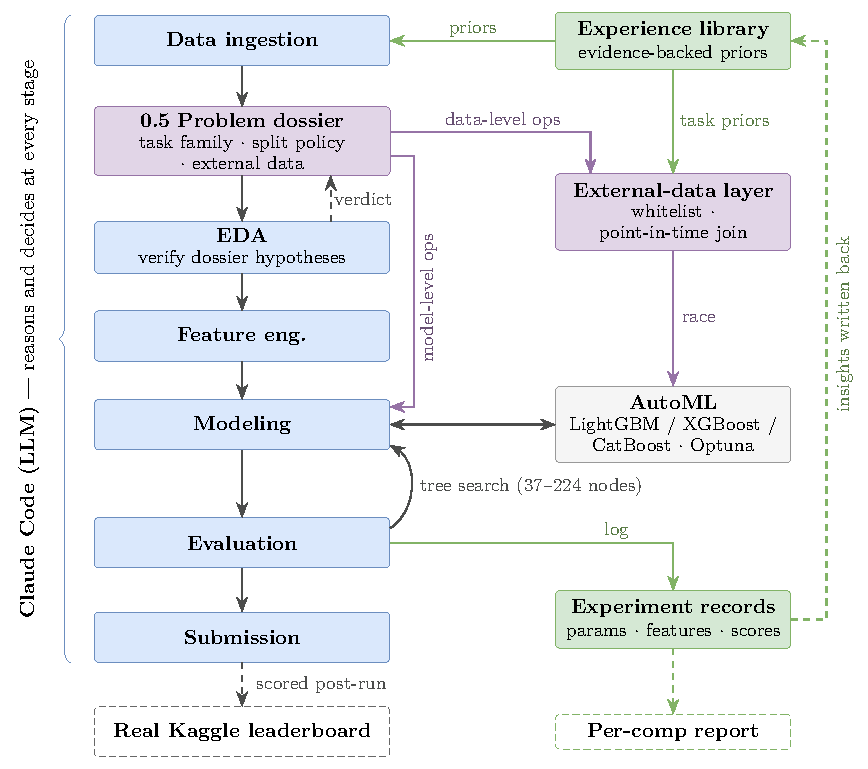
\includegraphics[width=0.82\linewidth]{fig1_arch.pdf}
\caption{Architecture of the Sinica Kaggle Agent, with color marking roles. \textbf{Blue, the LLM-driven pipeline}: Claude Code reasons and decides at every stage, and EDA records a verdict on the dossier's hypotheses (the dossier is a prior, not a conclusion). \textbf{Purple, the injection layer} (Section~\ref{sec:v5}): the Stage-0.5 dossier emits typed operators; data-level ones feed the external-data layer's arms, which race a no-external baseline with the winner taking the full budget, and model-level ones enter search lineages directly. \textbf{Green, the evidence loop}: the experience library and the experiment records, with validated insights written back. \textbf{Gray, AutoML tools} invoked via the shell. Dashed arrows mark feedback, advisory, or post-run steps. The leaderboard is external to the agent: lanes hold no credentials, and submissions are scored only after the run.}
\label{fig:arch}
\end{figure}

\paragraph{Tree-search protocol.} Every ordinary-competition run in this report uses the tree-search harness of Figure~\ref{fig:tree} (\path{tree_search/harness_v3.py}); none of the benchmark submissions here used the earlier downstream variant of that harness, whose measured near-null effect motivated the upstream layer (Section~\ref{sec:v5}).

\begin{figure}[htbp]
\centering
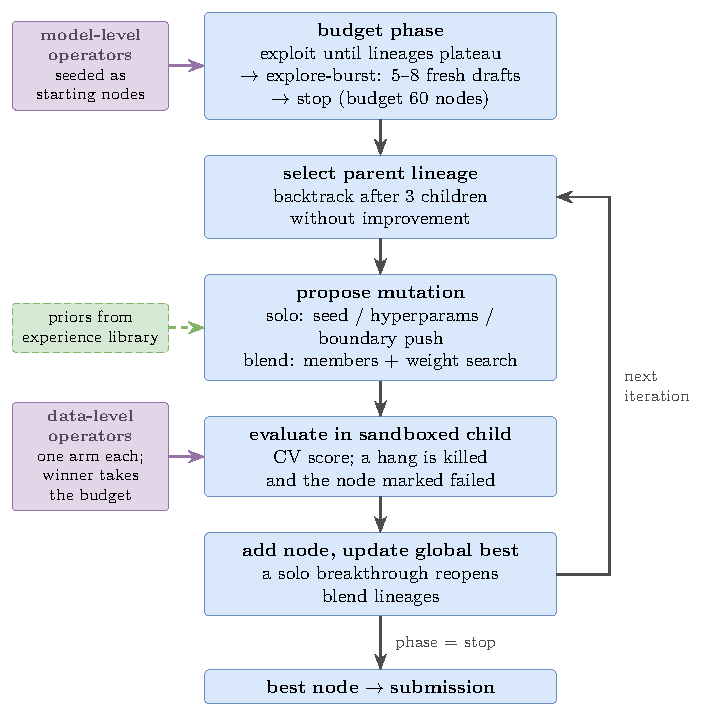
\includegraphics[width=0.6\linewidth]{fig2_tree_poster.pdf}
\caption{The tree-search loop used in all Sinica runs of this report (37--224 evaluated nodes per
competition). Each node is a complete, executable solution scored by local cross-validation:
lineages grow from the linear-protocol baseline, a lineage that fails to improve for three
children is abandoned, blends over cached out-of-fold predictions are first-class nodes, and the
best node becomes the submission. Purple: the injection layer's operator entry points
(Section~\ref{sec:v5}); green: priors from the experience library; dashed arrows: advisory input
and backtracking.}
\label{fig:tree}
\end{figure}

\subsection{The Injection Layer}
\label{sec:v5}

The purple elements of Figures~\ref{fig:arch} and~\ref{fig:tree} form a single layer, and its placement carries the design argument. An earlier downstream variant injected external ideas at the blend stage and measured a gain of only ${\sim}10^{-5}$ on the blend's competition metric; the architecture moves the injection point upstream to problem identification.

\paragraph{Stage 0.5: problem dossier.} Before EDA, the agent answers ``what kind of problem is this?'': task family, train--test window relation, split policy, and external-data need, written to \path{dossier.json}. Judgments are grounded in \path{knowledge/task_priors.md}, a library of task-level priors, each carrying an evidence field from our own benchmark. Reading competition-specific discussions or kernels is forbidden. The dossier must derive from the problem statement plus task-\emph{type} knowledge only, keeping the method distinct from reproduction-based agents. The dossier is a prior, not a conclusion: EDA must verify its hypotheses and record a verdict.

\paragraph{External-data module.} A whitelist of public sources, joined through leakage-guarded as-of merges: an external value may reach a prediction row only if dated at or before the row's period minus a declared lag. The module was adversarially audited; the flaws the audit surfaced and reproduced, including silent-future-leak classes, were fixed under regression tests. The dossier and the external-data module communicate through one closed vocabulary of typed operators, so a proposal the module cannot realize leaves a trace in a coverage ledger instead of being silently recorded as success. In controlled arms on the three \emph{firing-class} competitions, those where the layer fires by proposing external data (s3e19, tps-sep-2022, s5e1), all six external-data arms beat their matched no-external baselines on the private leaderboard, and the full s3e19 ablation, disabling the layer in the otherwise identical pipeline, moves the private score from $48.243$ to $50.455$; full arm scores are in the companion documents (see the Appendix).

\subsection{The Two Reference Agents}

\textbf{AIDE} (first-generation open-source release) performs LLM-driven tree search: at each step, it writes a complete solution, executes it, reads the error or score, and mutates accordingly. It carries no cross-competition memory. Every competition starts from zero.

\noindent\textbf{NVIDIA Kaggle Agent} (skill) reproduces the strongest public kernel: it researches the competition context, selects the highest-\emph{voted} solution-type kernel, ports it faithfully, and retrains on local data.

Both reference methods are frozen, with no improvements, even where we found weaknesses (the NVIDIA skill ships a score-based selection tool we deliberately left disabled). They stay frozen because improving a reference agent mid-study would make earlier and later data incomparable and would quietly turn the benchmark into an optimization of the reference methods.

\section{Benchmark Design}
\label{sec:fairness}

\paragraph{Evaluation set.} The study uses 23 competitions in two groups, mirroring the two scoring routes available. The 20 \emph{ordinary} competitions are tabular Kaggle competitions with live late submission: 7 classification tasks (binary and ordinal) and 13 prediction/regression tasks including time series and multi-target, with training sets from $1{,}157$ to $630{,}000$ rows. The 3 \emph{special} competitions sit outside the tabular family: us-patent (NLP text pairing), ventilator-pressure-prediction (physiological time series), and SIIM-ISIC melanoma (dermoscopic imaging); they are prepared and graded offline by MLE-bench~\cite{mlebench}, which replays finished Kaggle competitions with their original data and metrics.

\paragraph{Execution conditions.} The three agents ran serially on one machine, each method ``as shipped'': AIDE with its default 20 steps, NVIDIA reproducing public kernels per its method, Sinica running the full six-stage pipeline including tree search (37--224 evaluated nodes per competition). Four isolation conditions -- data, workspace, instruction, and resource -- are explicitly enforced rather than left to convention, and a fifth rule governs the experimenter, not the agents: when the environment is defective, fix the environment, never hint to the affected side (enforcement details in the Appendix).

\paragraph{Sandboxes, audit, and scoring.} Sinica's 20 ordinary-competition lanes each ran in an isolated root holding no credentials (the Kaggle token is stripped, so a lane can neither consult the leaderboard nor submit), and a per-lane transcript audit reads every tool call before a score is accepted. Two attempts were discarded by that audit and re-run clean, s3e19 and tps-jan-2022; on s3e19 the clean re-run scores \emph{worse} on local CV than the tainted attempt, evidence that the contamination had conferred a real advantage, and the root cause, a shared knowledge library left writable, was fixed by mounting it read-only. Each lane freezes a \path{submission.csv} that a separate credentialed operator step submits and scores on the real leaderboard; the AIDE and NVIDIA scores are frozen leaderboard scores from late submission. No local CV is quoted as evidence in this report's tables, because local estimates cannot arbitrate between agents: on s3e19 a pooled out-of-fold SMAPE of 6.71 sat against a realized lane score of 49.41.

\section{Results}
\label{sec:results}

\subsection{The 20 Ordinary Competitions}

Table~\ref{tab:bench} gives the complete benchmark: public and private leaderboard scores for all three agents on all 20 ordinary competitions. \textbf{Sinica takes the best private score on 10 of the 20} (NVIDIA 7, AIDE 3).

\begin{table}[H]
\centering\footnotesize
\setlength{\tabcolsep}{3pt}
\caption{The complete 20-competition benchmark. All cells are public/private leaderboard
scores; \textbf{bold} marks the best \emph{private} score of the three (direction-aware).
Sinica's column comes from the credentialed operator scoring step. All three agents carry the
public-leaderboard percentile rank (PR) of their public score in parentheses; Sinica's were
computed from public-leaderboard snapshots (2026-08-24) under the same convention that
reproduces the reference agents' recorded ranks, except on s5e1 and tps-sep-2022, where the
reference PRs come from an earlier pull and are not strictly comparable. All 20 lanes are
complete, audited and scored.}
\label{tab:bench}
\begin{tabular}{@{}rllrrr@{}}
\toprule
\# & \textbf{Competition} & \textbf{Metric} & \textbf{Sinica LB (pub/priv)} & \textbf{NVIDIA LB (PR)} & \textbf{AIDE LB (PR)} \\
\midrule
1 & s3e1 & RMSE \dn & 0.55715/\textbf{0.55275} (77.1) & 0.55332/0.55550 (93.2) & 0.55899/0.55552 (81.0) \\
2 & s3e3 & ROC-AUC \up & 0.89449/0.87157 (30.6) & 0.93526/\textbf{0.89537} (66.8) & 0.88484/0.86863 (26.4) \\
3 & s3e5 & QWK \up & 0.57041/0.57223 (72.0) & 0.57515/0.56974 (75.7) & 0.59362/\textbf{0.58138} (79.8) \\
4 & s3e7 & ROC-AUC \up & 0.91127/0.90441 (74.3) & 0.91230/\textbf{0.90458} (78.1) & 0.90934/0.90109 (67.1) \\
5 & s3e9 & RMSE \dn & 11.84750/12.33192 (51.2) & 11.83399/\textbf{12.22913} (59.1) & 11.86657/12.30667 (44.5) \\
6 & s3e11 & RMSLE \dn & 0.29309/\textbf{0.29368} (76.6) & 0.29559/0.29624 (66.6) & 0.29389/0.29445 (73.3) \\
7 & s3e14 & MAE \dn & 343.43434/333.18611 (66.3) & 338.36524/\textbf{330.71616} (89.2) & 342.44918/332.31556 (71.2) \\
8 & s3e16 & MAE \dn & 1.33738/\textbf{1.33822} (95.1) & 1.33566/1.34001 (96.4) & 1.33920/1.34224 (91.4) \\
9 & s3e19 & SMAPE \dn & 49.11872/49.40878 (37.6) & 47.52145/\textbf{48.26558} (41.4) & 48.39715/48.34131 (40.1) \\
10 & s4e11 & Accuracy \up & 0.94195/\textbf{0.94107} (64.0) & 0.94136/0.94076 (52.8) & 0.94184/0.94056 (62.1) \\
11 & s5e10 & RMSE \dn & 0.05554/\textbf{0.05576} (81.2) & 0.05562/0.05588 (59.4) & 0.05555/0.05579 (78.9) \\
12 & s6e1 & Error \dn & 8.68844/\textbf{8.71516} (76.8) & 8.70480/8.73239 (69.5) & 8.69449/8.72191 (74.8) \\
13 & s6e2 & ROC-AUC \up & 0.95354/0.95505 (68.6) & 0.95348/0.95508 (63.0) & 0.95364/\textbf{0.95516} (76.5) \\
14 & afsis & MCRMSE \dn & 0.41902/\textbf{0.48917} (72.7) & 0.61276/0.69855 (18.8) & 0.45636/0.49861 (45.6) \\
15 & cat-in-the-dat & ROC-AUC \up & 0.80800/\textbf{0.80243} (72.6) & 0.77641/0.77084 (32.6) & 0.80790/0.80217 (70.3) \\
16 & conway & MAE \dn & 0.10313/\textbf{0.10414} (100.0) & 0.11094/0.11189 (96.5) & 0.10960/0.11065 (97.9) \\
17 & tps-aug-2022 & ROC-AUC \up & 0.58534/0.58930 (63.5) & 0.57920/0.58730 (43.0) & 0.58479/\textbf{0.59106} (60.5) \\
18 & tps-jan-2022 & SMAPE \dn & 4.58859/6.29895 (75.4) & 4.43958/\textbf{4.63651} (76.4) & 10.11598/10.66638 (28.9) \\
19 & s5e1 & MAPE \dn & 0.09076/\textbf{0.08401} (74.3) & 0.05726/0.14594 (69.3) & 0.12573/0.17917 (48.1) \\
20 & tps-sep-2022 & SMAPE \dn & 28.45070/28.49605 (13.6) & 4.77458/\textbf{5.48351} (80.3) & 5.78998/9.72095 (48.3) \\
\midrule
\multicolumn{3}{@{}l}{Median PR (range)} & 72.7 (13.6--100.0) & 68.0 (18.8--96.5) & 68.7 (26.4--97.9) \\
\bottomrule
\end{tabular}

\end{table}

PR is the share of that competition's public-leaderboard standings that the submission's public score would beat. It is an \emph{absolute} capability reference, separate from the relative ordering among the three: Sinica's median PR sits at the 72.7th percentile of all human teams, the two reference agents' near the 68th. The private column remains the basis for every win/loss verdict; PR is contextual only.

\subsection{The 3 Special Competitions}
\label{sec:special}

The three agents ran on the three special competitions, each under its frozen method and the same isolation protocol. None of the Sinica lanes ran the injection layer or tree search: a node here is a full deep-learning fine-tune, not a seconds-long GBDT refit, so all three lanes took the skill's documented fallback, one linear pass to a validated single model plus a blend. Grading is offline against MLE-bench's held-out private split; medal thresholds and the above-median flag come from the frozen leaderboard snapshot.

\begin{table}[H]
\centering\small
\caption{The 3 special competitions, graded by MLE-bench. \textbf{Bold} = best of the three; $\dagger$ = above the frozen leaderboard's median.}
\label{tab:special}
\begin{tabular}{@{}lllll@{}}
\toprule
\textbf{Competition} & \textbf{Metric} & \textbf{Sinica} & \textbf{NVIDIA} & \textbf{AIDE} \\
\midrule
us-patent & Pearson $r$ \up & \textbf{0.86658}$\dagger$ (silver) & 0.86160$\dagger$ (bronze) & 0.65821 \\
ventilator & MAE \dn & \textbf{0.16525} & 0.40093 & 0.34591 \\
SIIM-ISIC & AUC \up & \textbf{0.93529}$\dagger$ & 0.89822 & 0.88579 \\
\bottomrule
\end{tabular}
\end{table}

Sinica takes the three-way best on all three and the only above-median score on SIIM-ISIC (Table~\ref{tab:special}): a sweep across three unrelated task families, consistent with the advantage coming from pipeline discipline rather than tabular-specific tuning.

\subsection{The Standing, and Where the Losses Fall}

Counting best scores across all 23 competitions, \textbf{Sinica obtains the best performance, with 13 wins and 10 losses}; the two reference agents split the remaining 10, all on ordinary competitions (NVIDIA 7, AIDE 3; Table~\ref{tab:bench}). Sinica's sharpest losses both fall on the two competitions with a mature public solution: on tps-sep-2022, whose public baseline is of unusually high quality, both reference agents beat it (5.48 and 9.72 SMAPE against 28.50), and on tps-jan-2022 NVIDIA's reproduction of the known GDP-ratio solution beats Sinica 4.64 to 6.30. Reproduction dominates exactly where a strong public solution already exists; the search-based agents take the majority of the rest.

\section{Discussion}

\subsection{Comparing the Three Agents}

The differences lie not in tuning skill but in where knowledge comes from and how the next step is decided (Table~\ref{tab:threeway}).

\begin{table}[htbp]
\centering\footnotesize
\setlength{\tabcolsep}{4pt}
\caption{Design comparison of the three methods.}
\label{tab:threeway}
\begin{tabular}{@{}L{3.2cm}L{4.2cm}L{3.4cm}L{3.6cm}@{}}
\toprule
\textbf{Aspect} & \textbf{Sinica} & \textbf{AIDE} & \textbf{NVIDIA} \\
\midrule
Knowledge source & Cross-competition experience library (accumulating) & None (from zero each time) & Public kernels fetched fresh each time \\
Search strategy & Six-stage pipeline + tree search (37--224 nodes) & Tree-shaped trial and error, 20 steps & No search; faithful reproduction \\
Basis for next step & Experience-library priors + OOF diagnostics & Previous step's error or score & Highest-voted kernel \\
Validation rigor & Split chosen by task type; diagnostics tagged and excluded & No concept of split legality & Inherits the kernel's split \\
External data & Injection layer (typed operators, whitelisted sources) & Never considered & Inherited from the kernel \\
\bottomrule
\end{tabular}
\end{table}

The reference agents' wins track their knowledge source: reproduction where a mature public solution exists, search depth where none does. Sinica's edge is validation rigor and accumulated knowledge (on one competition it quarantined the same shuffled split that AIDE submitted; see the companion case studies), while its measured bottleneck was judgment at problem identification, the gap the injection layer was built to close.

\subsection{Disadvantages of the Agent-Based Approach}

Running one agent through 23 competitions and reading every transcript also documents where the approach falls short.

\begin{itemize}[leftmargin=*]
  \item \textbf{The agent is strong at coding, weak at judging.} The agent efficiently works through whatever problem it is given; it does not ask whether a change is worth making. This often leads to a poor design choice that yields bugs, and the cost surfaces only after results return, when the choice is expensive to unwind (the downstream injection variant of Section~\ref{sec:v5} is our own instance).
  \item \textbf{The agent can only target the local validation score.} Inside a lane, the leaderboard is unreachable by construction, so iteration optimizes cross-validation alone. As a result, the local validation score can look outstanding while the real leaderboard score is mediocre: s3e19's pooled OOF SMAPE of 6.71 against its realized 49.41 is the extreme case, and it is why no local CV number is quoted as evidence anywhere in this report.
  \item \textbf{The agent often buries the main question in detail.} AI-written reports put too much focus on technical details, drifting away from what the reader wants to know; every specification report attached to this study needed human editing for exactly this failure.
  \item \textbf{The agent has bad writing habits.} Redundant headings and reinvented terms come back draft after draft, and verifying and modifying them by hand is exhausting; unlike a score, prose quality has no automatic gate.
\end{itemize}

\subsection{Practical Advice for Building AI Agents for Data Science}
\label{sec:advice}

Three pieces of advice, each paid for by a measurement in this study.

\begin{itemize}[leftmargin=*]
  \item \textbf{Build an isolated environment before running the agent.} This prevents any access to the leaderboard or another run's files. Isolation must be structural (credentials stripped, roots separated, library mounted read-only), not behavioral: the one cross-lane contamination in this study came from a writable shared file, not from an agent breaking a rule it was given (Section~\ref{sec:fairness}).
  \item \textbf{Justify the design before building the pipeline.} This mitigates redesign cost and debugging time and avoids a full rerun of earlier competitions: an architecture change invalidates every lane run before it, and this benchmark archived seven partly-finished runs for exactly that reason.
  \item \textbf{Inject external knowledge before data modeling.} This often improves the score; if the external data are injected at the final step instead, the score shows almost no improvement (${\sim}10^{-5}$ in our downstream variant, against six-for-six controlled wins for the upstream layer, Section~\ref{sec:v5}).
\end{itemize}

\subsection{Limitations}
\label{sec:limitations}

\begin{itemize}[leftmargin=*]
  \item \textbf{The sample is small and the standing is sensitive to its composition}: reproduction-based and search-based methods win on disjoint kinds of competitions, so adding or removing a few competitions of one kind moves the win count. Reproduced kernels were also tuned by their authors against the realized public leaderboard, so the comparison is least symmetric exactly where the reproduction method is strongest.
  \item \textbf{The special-competition lanes ran the documented fallback, not the full method} (Section~\ref{sec:special}), and offline grading yields one score per submission, with no public/private pair to corroborate it.
\end{itemize}

\subsection{Open Problems}
\label{sec:future}

The sharpest open question is operator-form selection: none of the three local signals we tested selects the form the injection should take, and one selector was killed by its own pre-registered test on s5e1. A fourth candidate, horizon length, emerged only after the fact; we have committed it as a pre-registration, to be tested on the next firing-class competition before its leaderboard is consulted. Second, few competitions need external data at all, so the controlled evidence rests on three firing-class competitions, only two of which (tps-sep-2022 and s5e1) played no part in building the task-prior library the dossier consults; extending that set is worth more than re-running competitions where the layer stays silent. Third, the experience library's residual weak link is retrieval quality: enforcement is closed (an experiment record without a library-query trace is invalid, checked mechanically), but no mechanism yet scores retrieved priors for applicability, and a direct ablation of the library remains to be run.

\section{Conclusion}

All 23 competitions ran in isolated sandboxes, the 20 ordinary ones transcript-audited and scored on the real leaderboard, the 3 special ones graded offline by MLE-bench. Among the 23 competitions, Sinica obtains the best performance, with 13 wins and 10 losses: the best private score on 10 of 20, and the three-way best on all 3 special competitions. Its losses concentrate where a mature public solution exists and reproduction beats search. The architectural answer is placement: the downstream injection measured a near-null effect, so knowledge enters at problem identification, and the layer's controlled evidence, scored on the leaderboard, carries the claim. Two negative results accompany the study: no local signal selects the injection's form, and the audit discarded a contaminated lane whose tainted score looked better than its clean replacement's. This study aimed to build a benchmark that can kill its own hypotheses.

\clearpage
\appendix

\section*{Appendix: Experimental Procedure and Availability}

\paragraph{Fairness protocol.} Because the three agents share one machine, four isolation conditions are explicitly enforced -- two by tooling, one by directory structure, and one, instruction isolation, by a written protocol with an incident log (Table~\ref{tab:fairness}).

\begin{table}[htbp]
\centering\small
\caption{The four isolation conditions and what enforces each.}
\label{tab:fairness}
\begin{tabular}{@{}L{2.6cm}L{6.4cm}L{5.6cm}@{}}
\toprule
\textbf{Condition} & \textbf{Rule} & \textbf{Enforcement} \\
\midrule
Data & Each side reads only its own root, containing files validated against the official Kaggle manifest & \path{build_isolated_roots.py} \\
Workspace & The three output directories are fully separated; each side is scored independently & Directory structure \\
Instruction & Prompts may carry environment facts and metric thresholds only: no modeling recipes, no other side's scores, no workaround discovered by another side & Manual protocol + incident log \\
Resource & Only one lane executes at any moment & \path{lane_lock.sh} mutex \\
\bottomrule
\end{tabular}
\end{table}


\paragraph{Per-competition specification reports.} Specification reports accompany this paper for all 23 Sinica runs (the 20 ordinary competitions, plus the 3 special competitions via a deep-learning-aware collector whose DL fields -- backbone, learning-rate schedule, batch size, augmentation, transfer learning -- are filled natively), along with 13 reports re-documenting the benchmark AIDE runs. All are written to the five sections of Tso-Jung Yen's ML specification framework -- Data / Models \& Architecture / Training / Inference / Evaluation \& Benchmarking -- archived in \path{docs/ml_specs/} and \path{benchmark_results/ml_specs_aide/} in Markdown and PDF. Every number in them is extracted deterministically by \texttt{collect.py} / \path{collect_aide_facts.py} from structured records, never generated by an LLM; unavailable fields are marked ``not recorded.'' The reports are CV-only by construction; their conclusions must not be mixed with leaderboard verdicts.

\paragraph{Execution environment.} All lanes ran on ARM64 Linux (Ubuntu 24.04) with an NVIDIA GB10 GPU, under a uv-managed Python 3.13 environment frozen in \texttt{uv.lock}, with fixed seeds and LightGBM set to \texttt{deterministic=true}, \path{force_row_wise=true} and a fixed \path{num_threads}; without these settings, the same configuration does not reproduce across processes.

\paragraph{Companion documents and availability.} Two companion documents carry the depth this report condenses: \emph{Building the Injection Layer: An Engineering Log} (per-regime coverage tables, audit scripts, and the provenance of the two special-competition scores that had to be re-run) and \emph{Per-Competition Case Studies} (the CV--leaderboard reversal mechanics, AIDE's split switch, the s5e1 pre-registration setting, and the s3e19 residual decomposition). All code and benchmark artifacts are archived in \href{https://github.com/930731haohao-afk/kaggle-agent}{\path{github.com/930731haohao-afk/kaggle-agent}} (private; access granted on request); every number in this report traces to those structured records.

{\small
\begin{thebibliography}{9}
\bibitem{aide2025} Jiang, Z., Schmidt, D., Srikanth, D., Xu, D., Kaplan, I., Jacenko, D., and Wu, Y. AIDE: AI-Driven Exploration in the Space of Code. arXiv:2502.13138 (2025).
\bibitem{aygun2026} Ayg\"un, E., et al. An AI system to help scientists write expert-level empirical software. \emph{Nature} \textbf{654}, 909 (2026). \url{https://doi.org/10.1038/s41586-026-10658-6}
\bibitem{nvidia2026} NVIDIA. Kaggle Agent: kernel-reproduction agent skill (software), 2026. \url{https://github.com/NVIDIA/nvidia-kaggle}
\bibitem{mlebench} Chan, J.\,S., et al. MLE-bench: Evaluating Machine Learning Agents on Machine Learning Engineering. In \emph{Proceedings of the 13th International Conference on Learning Representations}, 2025. \url{https://openreview.net/forum?id=6s5uXNWGIh}
\end{thebibliography}}

\end{document}
